%%%%%%%%%%%%%%%%%%%%%%%%%%%%%%%%%%%%%%%%%
% Journal Article
% LaTeX Template
% Version 1.3 (9/9/13)
%
% This template has been downloaded from:
% http://www.LaTeXTemplates.com
%
% Original author:
% Frits Wenneker (http://www.howtotex.com)
%
% License:
% CC BY-NC-SA 3.0 (http://creativecommons.org/licenses/by-nc-sa/3.0/)
%
%%%%%%%%%%%%%%%%%%%%%%%%%%%%%%%%%%%%%%%%%

%----------------------------------------------------------------------------------------
%	PACKAGES AND OTHER DOCUMENT CONFIGURATIONS
%----------------------------------------------------------------------------------------

\documentclass[twoside]{article}

\usepackage{lipsum} % Package to generate dummy text throughout this template

\usepackage[sc]{mathpazo} % Use the Palatino font
\usepackage[T1]{fontenc} % Use 8-bit encoding that has 256 glyphs
\linespread{1.05} % Line spacing - Palatino needs more space between lines
\usepackage{microtype} % Slightly tweak font spacing for aesthetics

\usepackage[hmarginratio=1:1,top=32mm,columnsep=20pt]{geometry} % Document margins
\usepackage{multicol} % Used for the two-column layout of the document
\usepackage[hang, small,labelfont=bf,up,textfont=it,up]{caption} % Custom captions under/above floats in tables or figures
\usepackage{booktabs} % Horizontal rules in tables
\usepackage{float} % Required for tables and figures in the multi-column environment - they need to be placed in specific locations with the [H] (e.g. \begin{table}[H])
\usepackage{graphicx}
\usepackage[hyphens]{url}
\usepackage{hyperref} % For hyperlinks in the PDF
 
\usepackage{lettrine} % The lettrine is the first enlarged letter at the beginning of the text
\usepackage{paralist} % Used for the compactitem environment which makes bullet points with less space between them

\usepackage{abstract} % Allows abstract customization
\renewcommand{\abstractnamefont}{\normalfont\bfseries} % Set the "Abstract" text to bold
\renewcommand{\abstracttextfont}{\normalfont\small\itshape} % Set the abstract itself to small italic text

\usepackage{titlesec} % Allows customization of titles
\renewcommand\thesection{\Roman{section}} % Roman numerals for the sections
\renewcommand\thesubsection{\Roman{subsection}} % Roman numerals for subsections
\titleformat{\section}[block]{\large\scshape\centering}{\thesection.}{1em}{} % Change the look of the section titles
\titleformat{\subsection}[block]{\large}{\thesubsection.}{1em}{} % Change the look of the section titles

\usepackage{datetime}


\usepackage{fancyhdr} % Headers and footers
\pagestyle{fancy} % All pages have headers and footers
\fancyhead{} % Blank out the default header
\fancyfoot{} % Blank out the default footer
\fancyhead[C]{Running title $\bullet$ \monthname\ 2015}
\fancyfoot[RO,LE]{\thepage} % Custom footer text

%----------------------------------------------------------------------------------------
%	TITLE SECTION
%----------------------------------------------------------------------------------------

\title{\vspace{-15mm}\fontsize{24pt}{10pt}\selectfont\textbf{RFID Based Bicycle Locking System}} % Article title

\author{
\normalsize
\textsc{Antal J. Monori, Emil M. Einarsson, Gustavo S. Buschle, Thomas T. Enevoldsen} \\[2mm] % Your name
\normalsize Aalborg Universitet \\ % Your institution
\normalsize \textit{<amonor14,eeinar14,gbusch14,tten14>}@students.aau.dk % Your email addresses
\vspace{-5mm}
}
\date{}

%----------------------------------------------------------------------------------------

\begin{document}

\maketitle % Insert title

\thispagestyle{fancy} % All pages have headers and footers

%----------------------------------------------------------------------------------------
%	ABSTRACT
%----------------------------------------------------------------------------------------

\begin{abstract}

\noindent Thi article focuses on how bicycle sheds in Denmark can be improved to reduce theft. Bicycles are stolen from public places such as schools and train stations because they are not secured to the surroundings and can therefore lifted from their parked location. The suggested solution attempts to encourage the users to use a supplied chain-locking system that allows the users to lock their bicycles to the modified racks. The prototype uses RFID technology to associate the user with the locked bicycle. The system uses a solenoid to operate the locking mechanism and a chain that is connected to the racks. The report concludes that RFID is a viable option for securing bicycles against the given issue.

\end{abstract}

%----------------------------------------------------------------------------------------
%	ARTICLE CONTENTS
%----------------------------------------------------------------------------------------

\begin{multicols}{2} % Two-column layout throughout the main article text

\section{Introduction}

\lettrine[nindent=0em,lines=3]{B}icycles are a popular means of travelling in several different countries around the world. In 2013, bicycles outsold passenger cars in almost every European country~\cite{outselling}. This popularity also requires well implemented and state-wide bicycle infrastructure, in which fortunately Denmark is one of the front-runners in Europe and around the world~\cite{impressive}. Parking spaces for bicycles are quite common in cities and around offices, public parks and government institutions. As bicycle sheds are freely accessible, and usually with no surveillance, it is easy to steal bicycles from within, due to the fact that the bicycles are not locked optimally.

According to the Danish Bank of Statistics, there has been reported an average of 540,599 bicycle theft incidents since 2007~\cite{bikestats}. Bicycles are most vulnerable to theft when left at public locations such as train stations, bus stations, in front of malls or even at public schools.


Factory new bicycles usually come fitted with some sort of locking mechanism. This allows the user to lock the bicycle at any given location, the limitations of the default lock usually do not allow the bicycle to be locked to the surroundings, leaving the bicycle vulnerable to being moved or taken even though it is locked. In Denmark, organised bicycle crime is common and thieves often steal large quantities of bicycles from public locations during every hour of the day. There has been multiple reports by Danish news establishment about public schools having issues with thieves stealing the pupils bicycles. These thieves steal truckloads of locked bicycles from sheds, schools and other public places, and then drives them to a foreign country. There, they easily remove the locks and the bicycles are sold or stripped for parts~\cite{herhuggerde}~\cite{vorescykler}. This means that bicycles of every price class are vulnerable to being stolen, since brand new bicycles are sold as they are and older bicycles are just stripped for parts and sold individually.


Reports have shown that this issue is preventable, but it requires more media coverage and attention. The government and other organizations throughout the world also need to be better at raising awareness on the issue of bicycle theft and should supply better designed bicycle racks, sheds and other solutions that serve as theft prevention. 

%------------------------------------------------

\section{Methods}

During the research for this project, we have figured out which technologies we will use when solving our problem statement. Through research we have looked at the different stakeholders and also taken into account the different health and safety measures and the environmental impact.
We will be using RFID to monitor and keep track of the different users of the locking system, for this project we will be using passive RFID, since this is the technology used in our student cards and other forms of ID cards. This will make it easy for us to integrate this system into working environments, where some sort of ID system already is in place. 
We gathered some data from the bicycle sheds at Aalborg University Esbjerg, and seen that the mounted locks are the most commonly used locks in our sample. Besides seeing how popular the mounted lock is, we have also seen how the chain locks are used in an ineffective manner. The reason for this is that most of the bicycles are not equipped with locks able to secure themselves to the surroundings, since the most common type is the mounted lock.

The processing unit of our locking system will be a micro-controller, this micro-controller will handle the different inputs and outputs from the various components.
To create a working locking solution that will work in practice we will be using a 12V or 24V solenoid. The solenoid will be the electrical component that moves a pin, so that the lock is electro-mechanically locked and unlock. 
Micro-controllers do not output a high enough voltage and a current to drive a solenoid, therefore we will need to work around this by using a relay. The relay will be used as an electrical switch controlled by the micro-controller to turn the solenoid on and off.

The main limiting factor for us is time. In the time frame of this project we cannot build a full scope product, finding all the parts, ordering, and assembling them completely would take too long. Furthermore we do not have the tools to build a full scope product either. Hence we will build a prototype as a proof of concept.


For our prototype, we decided to use a one fail-closed solenoid as opposed to a fail-constant locking mechanism. Fail-closed solenoids are easier to operate, cheaper, and easy to find, but they are not as flexible. We will implement this locking mechanism on a 1:1 scaled bicycle rack.
This prototype will not have all the features we wish to have for the final product, but the the goal is to show the interaction between an RFID reader and a locking mechanism, through a micro-controller.


The scope of this project is to create a working and affordable prototype of the above delimited problem, that would showcase the main capabilities of the end product, and would validate the idea of solving the presented problem in the Problem Analysis chapter.

Through testing our hypothesis and by fulfilling the requirements displayed above, we will be able to determine whether or not the project is a success.

%------------------------------------------------

\section{Results}

\begin{figure}[H]
    \centering
    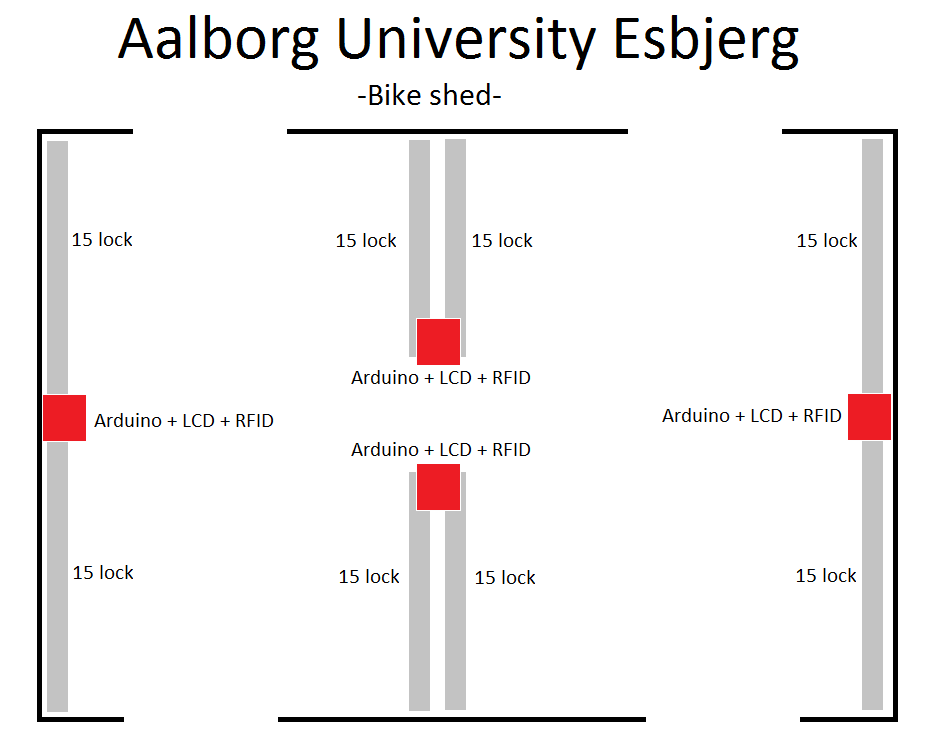
\includegraphics[width=0.5\textwidth]{./images/bikeshed.PNG}
    \caption{Aalborg University bike shed }
    \label{fig:bikeshed}
\end{figure}

Here is a basic concept idea of how we would implement the final design here in Aalborg University Esbjerg. For the final design a larger micro-controller would be necessary, like an Arduino MEGA, each MEGA could control up to 30 locks. All of the locks are controlled by a single RFID reader and one LCD screen. We would have our system on every other bicycle rack. So people could choose whether or not they wanted to use our system or their own locks.

The prototype case for the locking device is primarily built using plywood, a 12V solenoid, a mechanical relay, a switch and a Plexiglas cover.
 
The main prototype box contain an Arduino Uno development board (containing Atmel micro-comtroller), a RFID reader and a LCD 16x2 screen. They are placed in a ABS electrical box in which we have cut hole fitting the display. A RFID reader is located on the other side of the box, inside, under the label.

Both the locking enclosure and the case containing the micro-controller and electronic components are secured to a plywood wall and is mounted to the bicycle rack. The box containing the electronics is mounted on an extension that is tilted at an $45\,^{\circ}$ angle, making the display text more readable. The case containing the locking mechanism is mounted directly on the wall.

\begin{figure}[H]
	\centering
	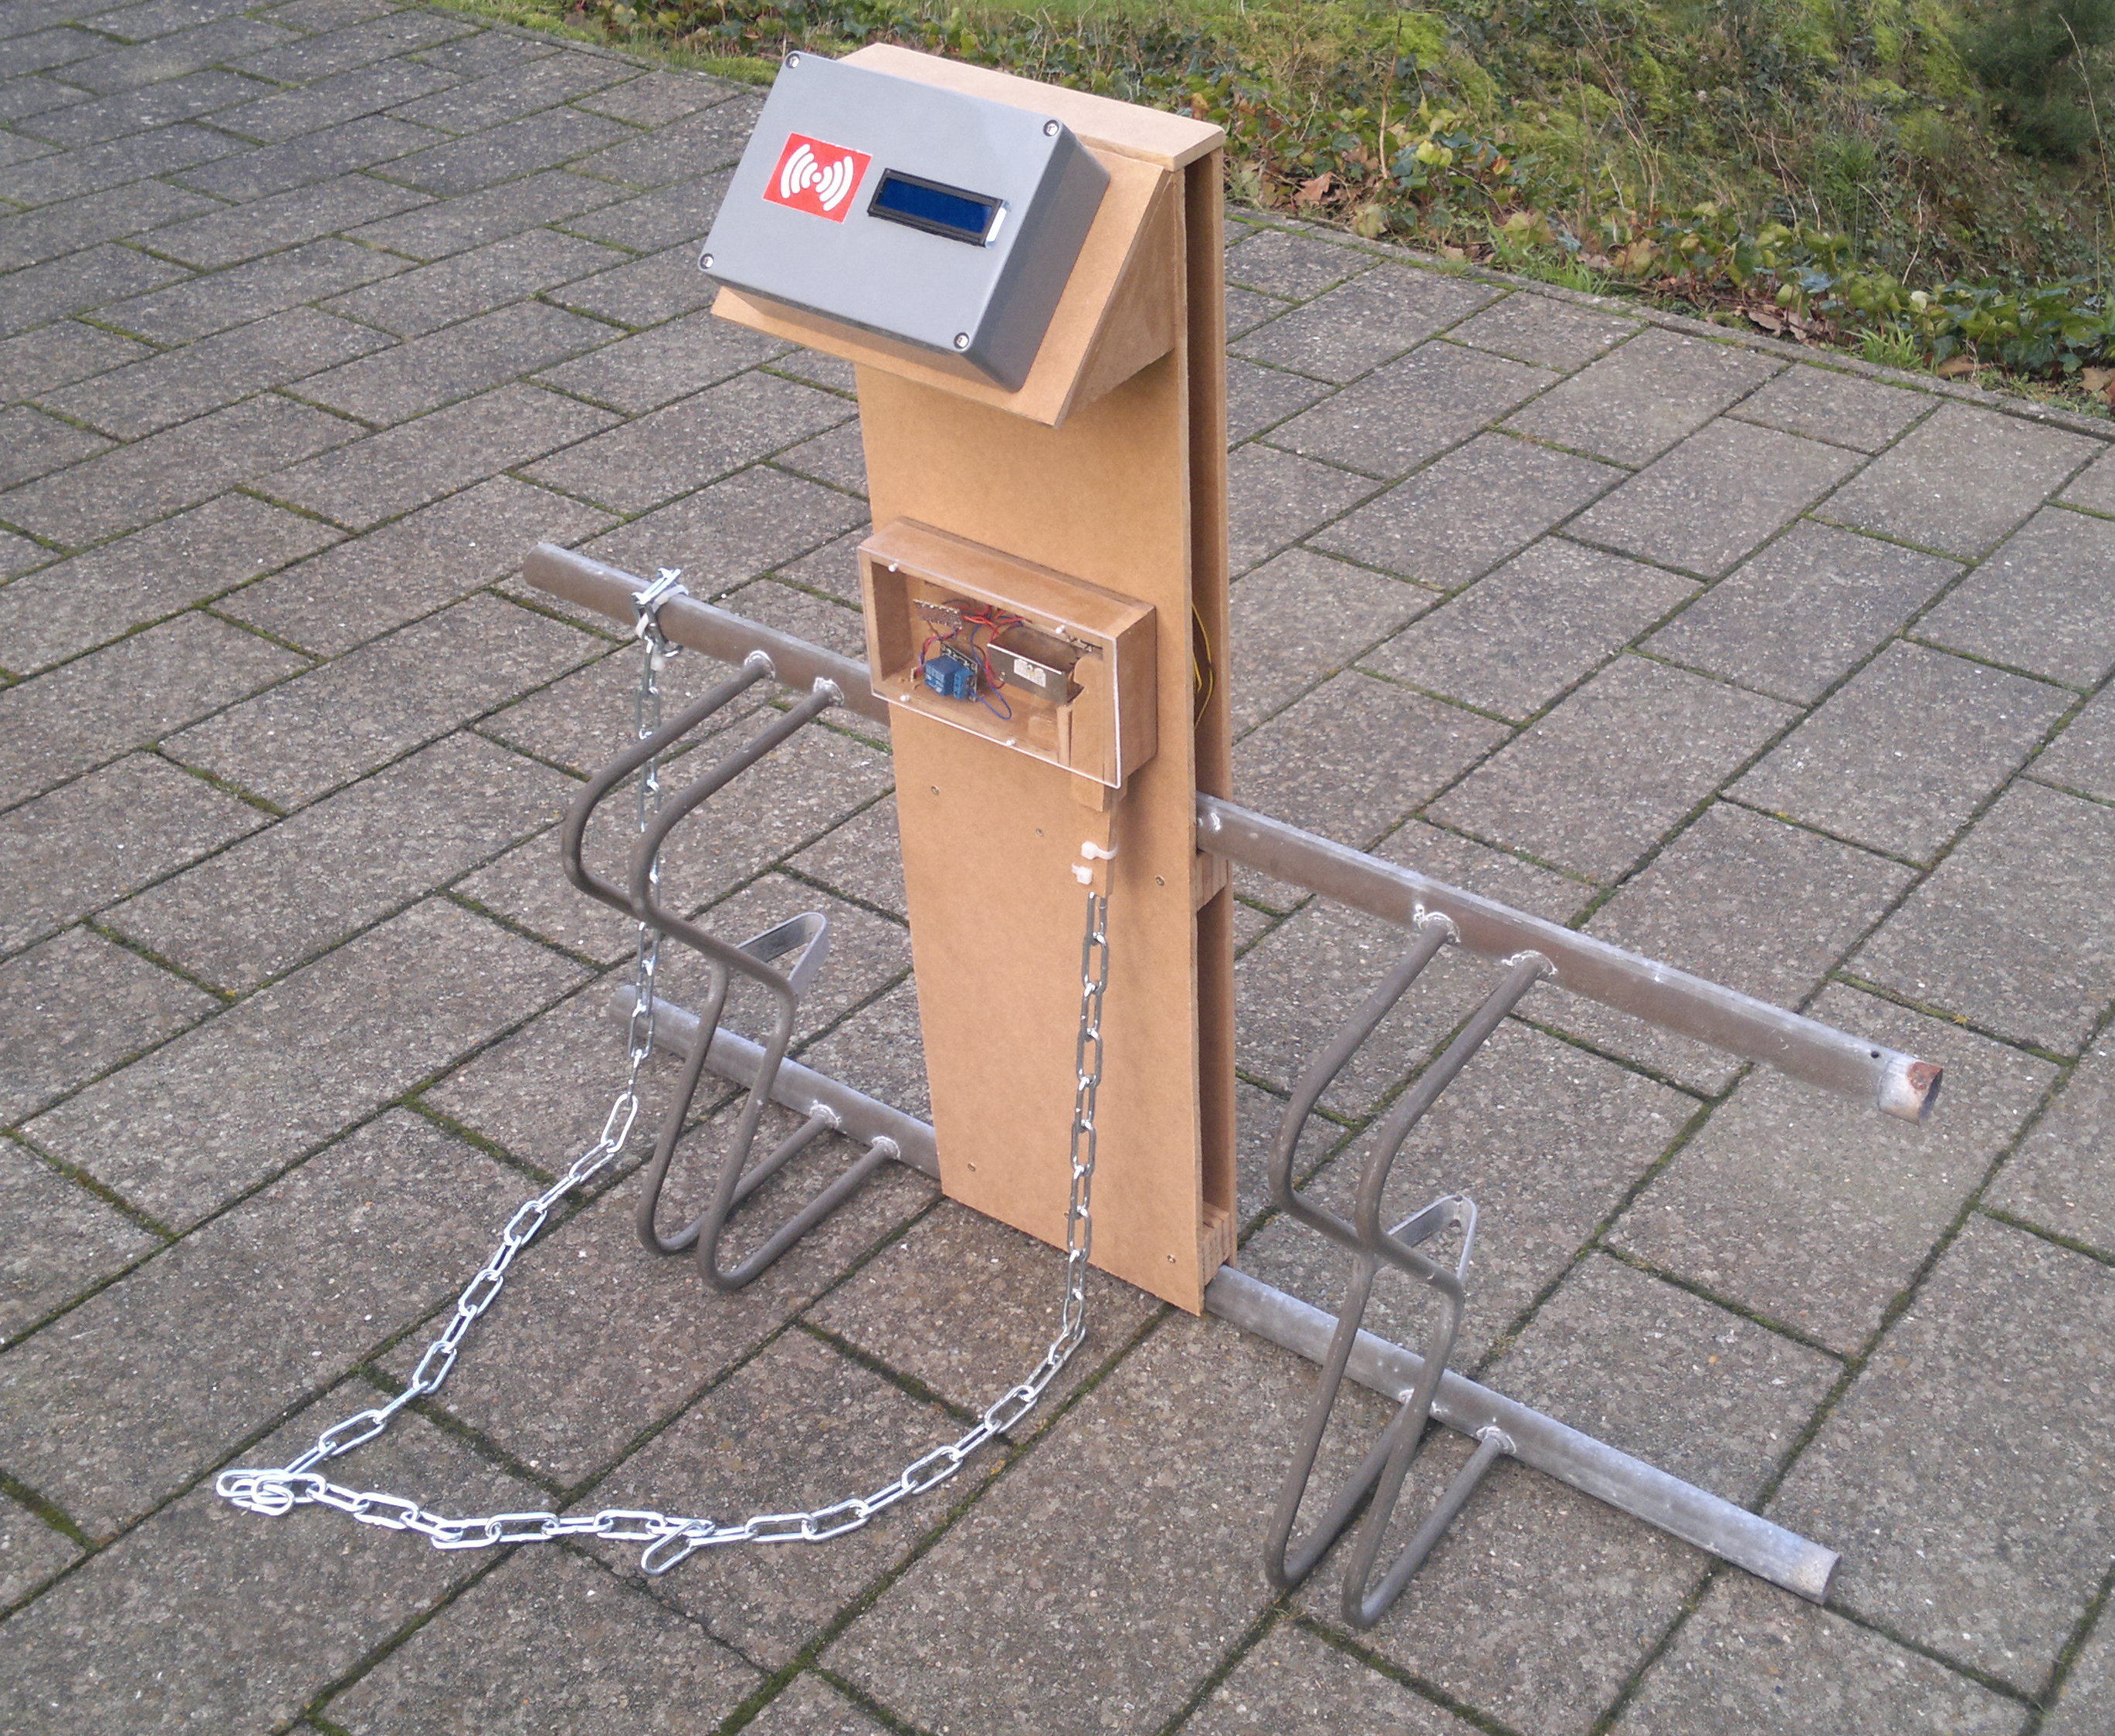
\includegraphics[width=0.5\textwidth]{images/full.jpg}
	\caption{Picture of prototype rack}
	\label{fig.rack}
\end{figure}

The components in the main box are connected by plug-in cables and soldered where needed, according to our design. The lock case and the wall is made of plywood using basic tools. The lock case construction is glued and nailed together, built after a slightly altered design, due to the fact that more advanced tools were not available. 

%------------------------------------------------

\section{Discussion}
The main purpose of this discussion is to take a look at our success criteria for our prototype and our hypothesis, to discuss the different results from our development and testing. In the problem definition, we created a hypothesis and defined a certain list of prototype and testing requirements. If these points are met, the prototype will be viewed as a success.

Our hypothesis is the following: 
\textit{The solution to the initiating problem implemented in this project, will make it harder for thieves to remove bikes from bicycle sheds due to inefficient locking by their owners. The solution in place will use RFID-based cards to lock their bicycles to the rack to reduce time spent on parking and reducing the stress level by preventing bicycle theft.}

To ensure that the hypothesis was thoroughly tested, we set up the prototype and testing requirements accordingly, so that we were sure that the different success criteria were met. 
We constructed a full-size prototype with a single lock, to get a realistic view of the design. This was to make sure that our suggested solution actually is feasible.

Below you will find a with list the prototype requirements.
\begin{enumerate}
	
	\item The model should be 1:1.
	\item It should operate sequentially.
	\item It should be operated by one person at a time.
	\item One micro-controller should only handle one lock.
	\item The system should include an RFID reader.
	\item It should be compatible with existing RFID cards.
	\item It should be using an Arduino single board micro-controller.
	\item The program should be written in C++ and C.
	\item The case for the lock and the lock should be made out of wood for easy prototyping.
	\item The lock should be stripped to the rack.
	\item The controller case should be pre-built.
	\item A display should be used to interact with the user.
	
\end{enumerate}

To achieve our prototype requirements, it was necessary for us to acquire a regular sized bicycle rack, so that the testing scale could be more realistic. The prototype is operated by a sequence of steps, that are clearly stated on the display. The prototype also has one lock, this fulfills the requirement with the number of locks the prototype should handle. And finally, the prototype is compatible with existing RFID cards, we mainly used our student cards to test the system with.


The prototype is user-friendly and clearly states the directions for use on the display. The materials used for the prototype have proven to be sturdy and give realistic feedback to what the setup might be able to endure during a larger scale field test.
After testing our prototype we can conclude that we have made functioning locking system, that allows a single user to lock their bicycle to the rack and associate it with their student ID card. Our prototype successfully demonstrates a single unit, where one user can access the device at a time. The larger scale implementation of this solution, is to use the same kind of display and card reader, but instead with greatly increased amount of locks along the bicycle rack. The built-in sensor would then recognize which lock has been locked, at intelligently associate it with a card. 


The different risks from the risk management have all be taken into consideration. Some of the risk are too big for our prototype scope, but they will be taken into consideration in the further development of the product.

\begin{figure}[H]
    \centering
    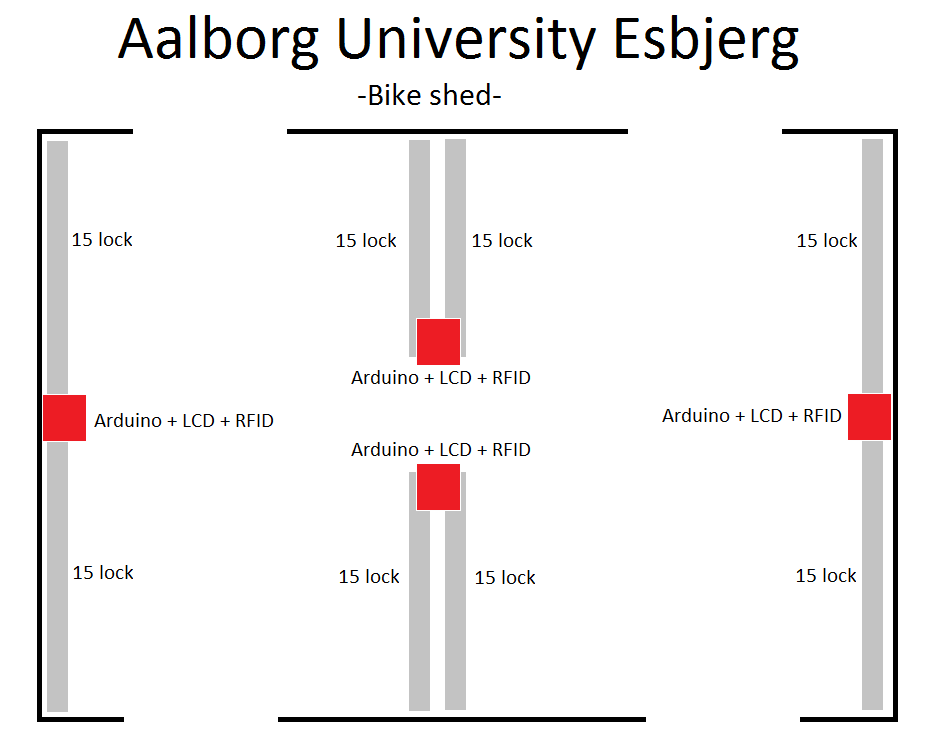
\includegraphics[width=0.6\textwidth]{./images/bikeshed.PNG}
    \caption{Aalborg University bike shed }
    \label{fig:bikeshed}
\end{figure}

The figure above shows how the single display and card reader would be associated with a greater number of locks.


One of the major flaws with our prototype is the actual security. The chain used to lock the bicycle to rack is vulnerable to wire cutters. But since this is a prototype, we do not consider this security risk as a failure, but instead it needs to be addressed in future versions. It would be necessary to take a deeper lock at using different materials needed to make a secure chain lock and to re-write the software so that there are no risk of exploits.
Since the RFID card reader reads every card type, it has the potential to steal peoples unencrypted data from their cards. This needs to be addressed in improved versions of the product, to avoid possible code manipulation in the product once it has been shipped.


We have successfully proven our hypothesis through our prototype. If the prototype is placed on the campus grounds, any given student at Aalborg University Esbjerg is able to lock their bicycle to the bicycle rack. This means that the bicycle in theory is not vulnerable to thieves carrying the bicycle away from its locked location. The prototype removes the inconvenience of carrying around a chain lock and encourages users to lock their bicycle to rack using the supplied setup.



%----------------------------------------------------------------------------------------
%CONCLUSION
%----------------------------------------------------------------------------------------
\section{Conclusion}
Based on the test results, we can conclude that our hypothesis stands correct, that picking up bicycles is harder when a proper bicycle-locking system is implemented. Our prototype validates the suggested solution, which is to implement an RFID-based locking mechanism on top of a bicycle rack. Throughout the analysis of the problem, we figured out that bicycle theft is a confirmed problem in Denmark due to the ineffective use of the existing bicycle racks. Using RFID technology for identification was a good choice, due to RFID is being widespread. Due to simplicity, of running the solenoid and the fact that we did not have to create any extra mechanical parts, easy accessibility, and running cost, we can conclude that the solenoid was a good choice for the locking mechanism, for the prototype and for future use.


Starting out by prototyping the individual components helped us to identify risks and potential issues. It helped us to identify the appropriate micro-controller, screen and libraries associated with them. We correctly limited the code to fit the scope of our prototype and to live up to the written requirements.


Building the prototype validates the suggested solution, which is to implement an RFID-based locking mechanism on top of a bicycle rack. 

%----------------------------------------------------------------------------------------
%----------------------------------------------------------------------------------------
%	REFERENCE LIST
%----------------------------------------------------------------------------------------
\bibliographystyle{unsrt}
\bibliography{citations}{}
%----------------------------------------------------------------------------------------

\end{multicols}

\end{document}
